\section{Overview of Mining GCMP in Parallel}
\label{sec:system_overview}
We adapt the MapReduce paradigm for designing
a parallel solution of mining GCMP. In this section,
we briefly describe the preliminaries on MapReduce and then describe
the overview of our framework in mining GCMP.

\subsection{Preliminary on MapReduce}
MapReduce (MR) was formally proposed by Dean et.al.~\cite{dean2008mapreduce}
and has subsequently implemented by many open source systems. Those systems
provide handy APIs with fault tolerances and are popularly
used as large-scale data processing platforms. 
% become a ubiquitous parallel platform for large-scaled data processing. 
%Current open source MapReduce systems provide handy programming APIs with fault tolerances
%in backends. Such systems include Hadoop, Shark and Spark to name a few.
In simple words, there are two conceptual types of computing nodes in MR,
namely the \emph{mapper}s and the \emph{reducer}s. The execution of a MR 
algorithm consists of three major steps: First, input data
are partitioned and read by a \emph{map} function on each mapper. Then, mappers
emit key-value pairs which are \emph{shuffle}d over the network to reducers. Lastly,
reducers process the received data using a \emph{reduce} function. 

Despite the simpleness of the paradigm, there are two concerns raised in designing MR algorithms
First, since reducers are required to be independent, partitioning  
data to fit the independence could be challenging. Second, since the \emph{shuffle}
step requires network access, the data been shuffled should be minimized. 
We take these concerns in consideration when designing our solutions for mining GCMP.
%We would bare this concerns in designing our GCMP mining algorithm.
%a natural
%problem is how to partition the data in map and shuffle phase so that reducers 
%achieve the independence.
%
%A critical question in designing a MapReduce algorithm is how to make 
%data partitions during the shuffle stage. In fact, a MapReduce algorithm 
%requires data processed at each reducer to be independent.
%
%Since the \emph{shuffle} stage needs to transfer data over network, 
%an important attention to pay during designing MapReduce an algorithm is 
%to minimize the shuffle amounts and shuffle counts. 

\subsection{MapReduce Processing for Mining GCMP}
Our GCMP mining process consists of two MR jobs as illustrated in Figure~\ref{fig:overview}.
The first MR job is to cluster objects at each snapshot (i.e.,
 $\forall t, o,$ compute $C_t(o)$). As shown in Figures~\ref{fig:overview}(a)-(b),
in map phase, trajectories are firstly reorganized by timestamps and object locations
at the same timestamps form a snapshot. In reduce phase, clustering of objects at each
snapshot is processed independently. The second MR job is to mine GCMPs from 
clusters in each snapshot. We design and compare two MR algorithms (i.e., TRM and SPM)for 
GCMP mining. Both the two algorithms would partition snapshots in map phase
(as in Figure~\ref{fig:overview}(c))
and mine GCMPs from each partition in reduce phase(as in Figure~\ref{fig:overview}(d)).

% corresponds to Figures~\ref{fig:overview}(a)-(b). The objective
%of the first job is to cluster trajectories based on snapshots (i.e.,).
%As illustrated in (a), input trajectories are read in by mappers 
%and are sprinkled into $\langle t,o \rangle$ pairs. In (b), objects with the same timestamp
%form a snapshot. Then, a user defined clustering method is applied on the objects
%in each snapshot in reducers. Between step (a) and (b), a shuffle is necessary. 
%The second
%MapReduce job corresponds to Figures~\ref{fig:overview} (c)-(d). The objective 
%of the second job is to mine the GCMP from the snapshots computed in the first job. We design
%two approaches (to be described shortly)for mining GCMP in parallel. In overview, as shown in (c), snapshots
%are first fed to mappers and different partition strategies may be selected to create
%partitions among snapshots. In (d), the partitions are then send to reducers to mine GCMP.
%The final computed results are then outputted to the end users. 

Although we need two MR jobs to complete the GCMP mining task, 
it is easy to pipeline the two jobs to exploit data locality.
Specifically, the reducer output at step (b) can be directly reused 
as the input to the mappers at step (c). Therefore we do not need to 
transfer data between the two jobs. Modern MR platforms, especially Spark, have
already supported such a kind of pipeline.

\begin{figure} [t]
\center
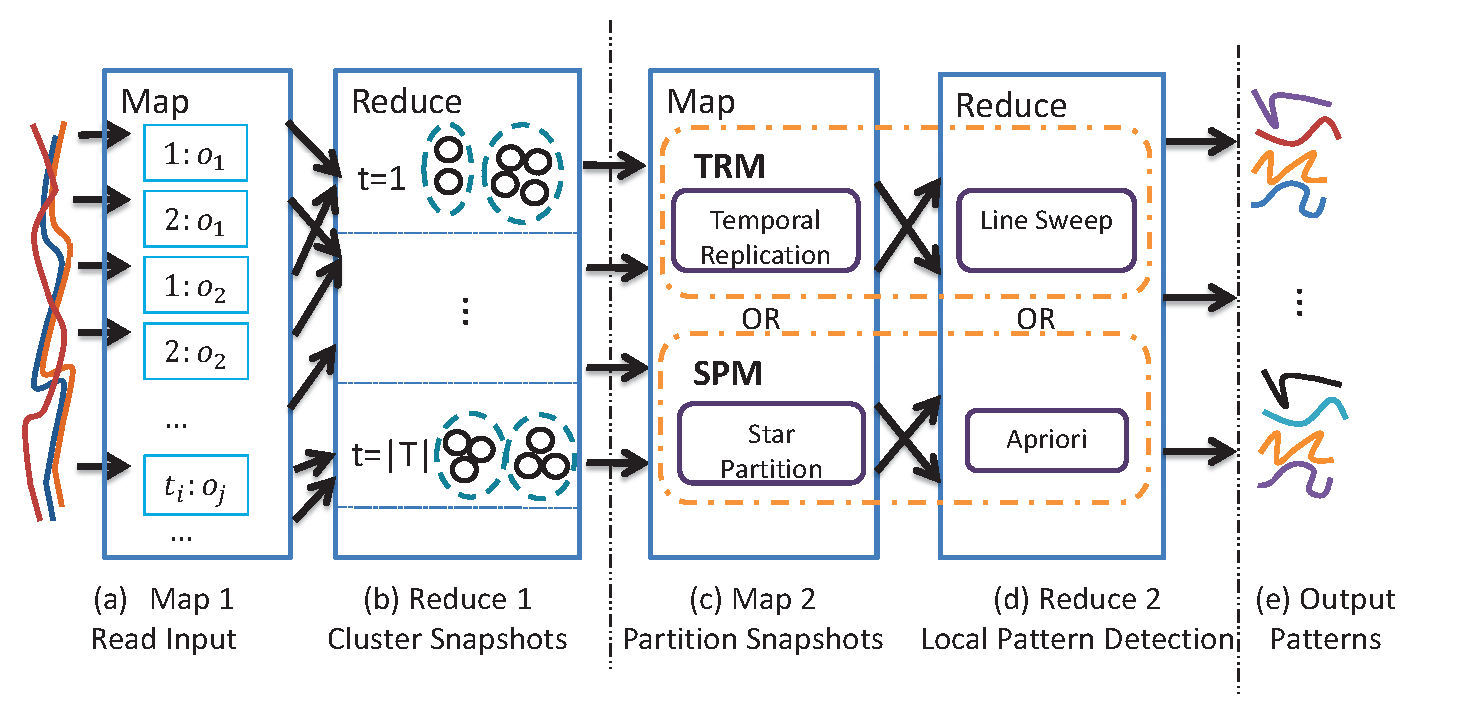
\includegraphics[width=0.5\textwidth]{system_layout.eps}
\caption{System flow of mining GCMP. (a)(b) correspond to the first MR job which compute the clusters at each snapshot; 
(c)(d) correspond to the second MR jobs which mines GCMP in parrallel.}
\label{fig:overview}
\end{figure}

We note that the first MR job is easy to design since each reducer only
needs one snapshot for clustering.
In contrast, it is challenging to design the second job. 
This is because valid patterns may spray across multiple snapshots 
or contain different object sets, where inappropriate partitioning
of snapshots may fail to discover certain valid patterns.
Formally, a valid partition strategy 
needs to meet the following requirements: (a) the resulted partitions need
to preserve enough information so that real patterns can be discovered in the reduce phase. 
(b) the resulted partitions need to ensure that
the patterns discovered in the reduce phase are valid patterns so that
no further verification is required. We formalize these two 
properties as \emph{completeness} and \emph{soundness} as follows:

\begin{definition}[Completeness and Soundness]
Let a partition method $\mathbb{P}$ partitions original trajectories $Tr$ into multiple parts, $Par_1,...,Par_m$. $\mathbb{P}$ is complete if for every pattern $P$ that is valid in $Tr$, $\exists Par_i$ s.t. $P$ is valid in $Par_i$. $\mathbb{P}$ is sound if for all patterns that are valid in any $Par_i$, they are also valid in $TR$.
\end{definition}
The completeness ensures that no true patterns are missed out. 
The soundness ensures that no false patterns are reported. 
If a partition method is both sound and complete, then it can be used
in the second MR job to facilitate GCMP mining.

Apparently, replicating the entire trajectories to each 
partition meets the \emph{soundness} and \emph{completeness} requirements. 
However, it burdens the network shuffle and limits the parallelism. 
Our objective is thus to design a complete and sound partition method that minimize the network shuffles.
In the following sections, we describe a naive \emph{temporal-based} partition-and-mining method called \emph{Temporal Replication and Mining}(TRM) towards a parallel solution of GCMP mining. Then,
we present a novel \emph{object-based} partition-and-mining method
called \emph{Star Partition and Mining} (SPM) which resolves
the deficiencies of TRM method.
